\chapter{7.9 习题}
%---------- 1 ----------------
\begin{flushleft}
1.修改“Shapes”演示以使用 GeometryGenerator::CreateGeosphere 而不是 GeometryGenerator::CreateSphere。 尝试使用0,1,2和3细分级别。\\
\end{flushleft}

%---------- 2 ----------------
\begin{flushleft}
2.修改“Shapes”演示以使用十六个根常量来设置每个对象的世界矩阵而不是描述符表。\\
\end{flushleft}

%---------- 3 ----------------
\begin{flushleft}
3.在DVD上,有一个名为 Models/Skull.txt 的文件。 该文件包含图\ref{fig:7-11}中渲染头骨所需的顶点和索引列表。 使用文本编辑器(如记事本)研究文件,并修改“形状”演示以加载和渲染头骨网格。\\
\end{flushleft}

\begin{figure}[h]
    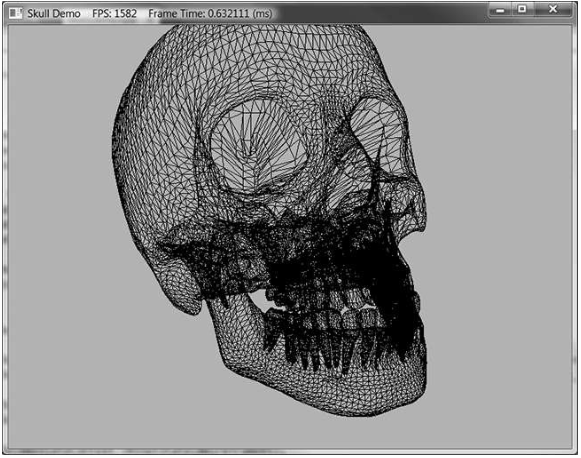
\includegraphics[width=\textwidth]{7-11}
    \centering
    \caption{练习3的渲染输出}
    \label{fig:7-11}
\end{figure}